\section{Res\_sample: A sample-like component for resolution calculation}
\label{s:res_sample}
\index{Samples!Resolution function, sample for}

\component{Res\_sample}{(System); Alan Tennant, HMI}{$r$, $r$, $h$, $r_{\rm focus}$, $x_{\rm target}$, $y_{\rm target}$, $z_{\rm target}$, $E_0$, $\Delta E$ }{$x_w$, $y_h$, $z_d$, $x_{\rm focus}$, $y_{\rm focus}$, $a_{\rm v, focus}$, $a_{\rm h, focus}$, target index}{}

The component \textbf{Res\_sample} scatters neutron rays isotropically
in direction and uniformly in energy.
Regardless of the state of the incoming neutron ray,
all directions and energies for the scattered ray have the same probability,
within specified intervals.

The component is meant
for computation of the resolution function, but may also be used
for test and debugging purposes. For actual calculations of the resolution
function, {\bf Res\_sample} should be used
together with \textbf{Res\_monitor}, described in
section~\ref{s:res_monitor}.

The shape of {\rm Res\_sample} is either a hollow cylinder
or a rectangular box.
The hollow cylinder shape is
specified with the outer radius, $r$ and thickness,
respectively, and the height, $h$.
If these parameters are unspecified,
the shape is instead a box of dimensions $x_w$, $y_h$, and $z_d$.
%
%\begin{figure}[htbp]
%  \begin{center}
%        \psfrag{ri}[c][c]{\textit{radius\_i}}
%        \psfrag{ro}[c][c]{\textit{radius\_o}}
%        \psfrag{h}[c][c]{\textit{h}}
%        \psfrag{bri}[c][c]{\textit{radius\_i}}
%        \psfrag{bro}[c][c]{$-\textit{radius\_o}$}
%        \psfrag{bh}[c][c]{\textit{h}}
%        \psfrag{X}[c][c]{\textit{X}}
%        \psfrag{Y}[c][c]{\textit{Y}}
%        \psfrag{Z}[c][c]{\textit{Z}}
%        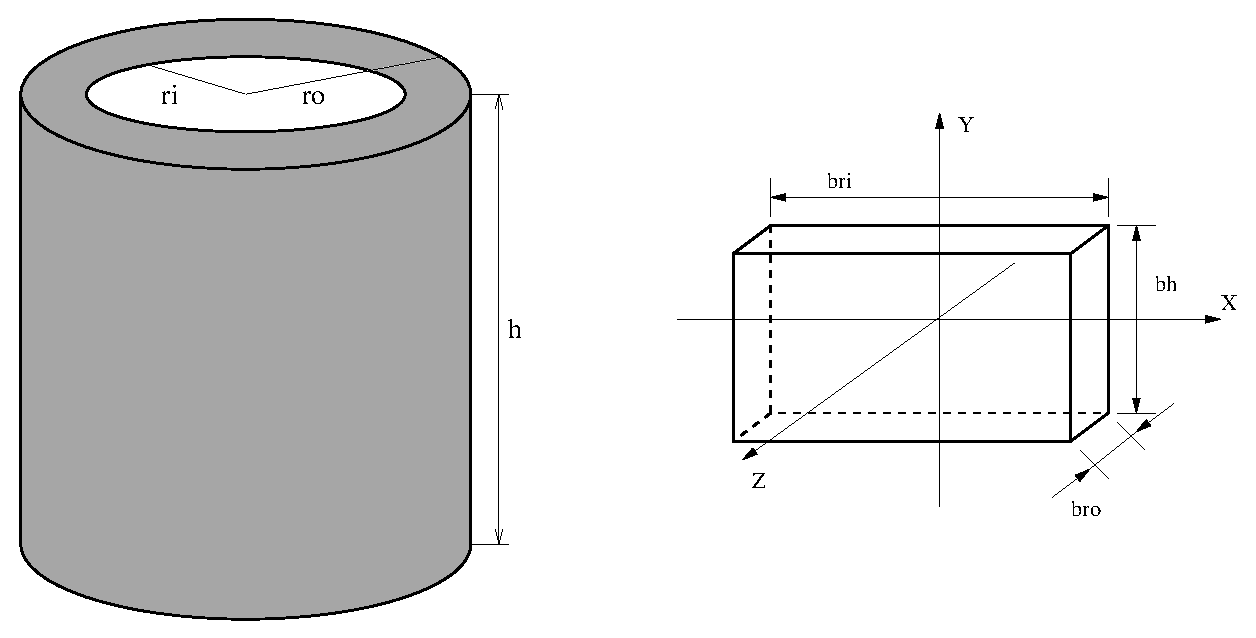
\includegraphics[width=0.9\textwidth]{figures/res_sample}
%    \caption{The two possible shapes of the \textbf{Res\_sample} component.}
%    \label{f:res_sample}
%  \end{center}
%\end{figure}
%
The component only propagates neutron rays that are scattered;
other rays are absorbed. The scattering probability is proportional to the neutron
flight path length inside the sample, to make a true volume weighting
of the sample. The reason for this is that the resolution
function of an instrument is independent of any sample properties
such as scattering and absorbtion cross sections but will in general
depend on sample size and shape.

The point of scattering inside the sample is chosen uniformly
along the neutron flight path inside the sample, and the scattered
neutron ray is given a random energy and direction. This energy is selected in
the interval $[E_0-\Delta E; E_0+\Delta E]$ which hence must be
chosen large enough to cover all interesting neutron energies.
Similarly, the scattered
direction is chosen in a user-specified range,
either within a sphere of radius $r_{\rm focus}$, within a rectangular
target with measures $(x_{\rm focus}, y_{\rm focus})$
or in the specified angular range. This target is positioned at the $x_{target}$, $y_{target}$, $z_{target}$ point in space, or using the target\_index for which e.g. 1 is the further component, -1 is the previous, etc...

A special feature, used when computing resolution functions, is that the
component stores complete information about the scattering event in the
output parameter \textit{res\_struct}. The information includes initial
and final wave vectors, the coordinates of the scattering point, and the
neutron weight after the scattering event. From this information the
scattering parameters $({\bf Q}, \omega)$ can be recorded
for every scattering event and used to compute the resolution function.
For an example of using the
information in the output parameter, see the description of the
\textbf{Res\_monitor} component in section~\ref{s:res_monitor}.

